% ============================================================
% Appendix A（既存）
% ============================================================
\chapter*{付録 A：Merton モデルにおける倒産距離の数学的導出}
\addcontentsline{toc}{chapter}{付録 A：Merton モデルにおける倒産距離の数学的導出}

本研究は Bharath \& Shumway（2008）が示したように、
Merton（1974）の倒産距離（Distance to Default: DD）構造を、
観測可能な proxy 変数へ写像するアプローチを採用している。
したがって本付録では、まず Merton モデルにおける倒産距離の数学的導出を整理し、
その後に本研究モデルとの対応関係を明確化することで、
理論的基盤と本研究の位置づけを統一的に示す。

\section*{A.1　Merton モデルの基本構造}
\addcontentsline{toc}{section}{A.1 Merton モデルの基本構造}

Merton（1974）の構造モデルでは、企業価値 $V_F(T)$ が満期 $T$ において



\[
V_F(T) < D
\]



となるとき企業は倒産すると定義される。ここで $D$ は負債額である。
企業価値は幾何ブラウン運動に従うため、対数変換した $\ln V_F(T)$ は正規分布に従う。
この性質により、倒産確率を正規分布の枠組みで扱うことが可能となる。

倒産条件 $\ln V_F(T) < \ln D$ を用いると、倒産確率は



\[
P\left( \ln V_F(T) < \ln D \right)
\]



として表される。ここで $\ln V_F(T)$ が正規分布に従うことから、
倒産確率は標準化された距離（倒産距離：DD）を用いて表現できる。

倒産距離 DD は次式で定義される。



\[
DD = \frac{\mathbb{E}[\ln V_F(T)] - \ln D}{\sqrt{\mathrm{Var}[\ln V_F(T)]}}
\]



これは、企業価値の対数が倒産閾値 $\ln D$ からどれだけ離れているかを
「標準偏差何個分か」で測る指標である。
DD が大きいほど倒産から遠く、DD が小さいほど倒産に近い。

正規分布の閉包性により、DD は標準正規分布に写像できるため、
倒産確率は



\[
P(\text{default}) = \Phi(-DD)
\]



として計算される。

\begin{figure}[H]
\centering
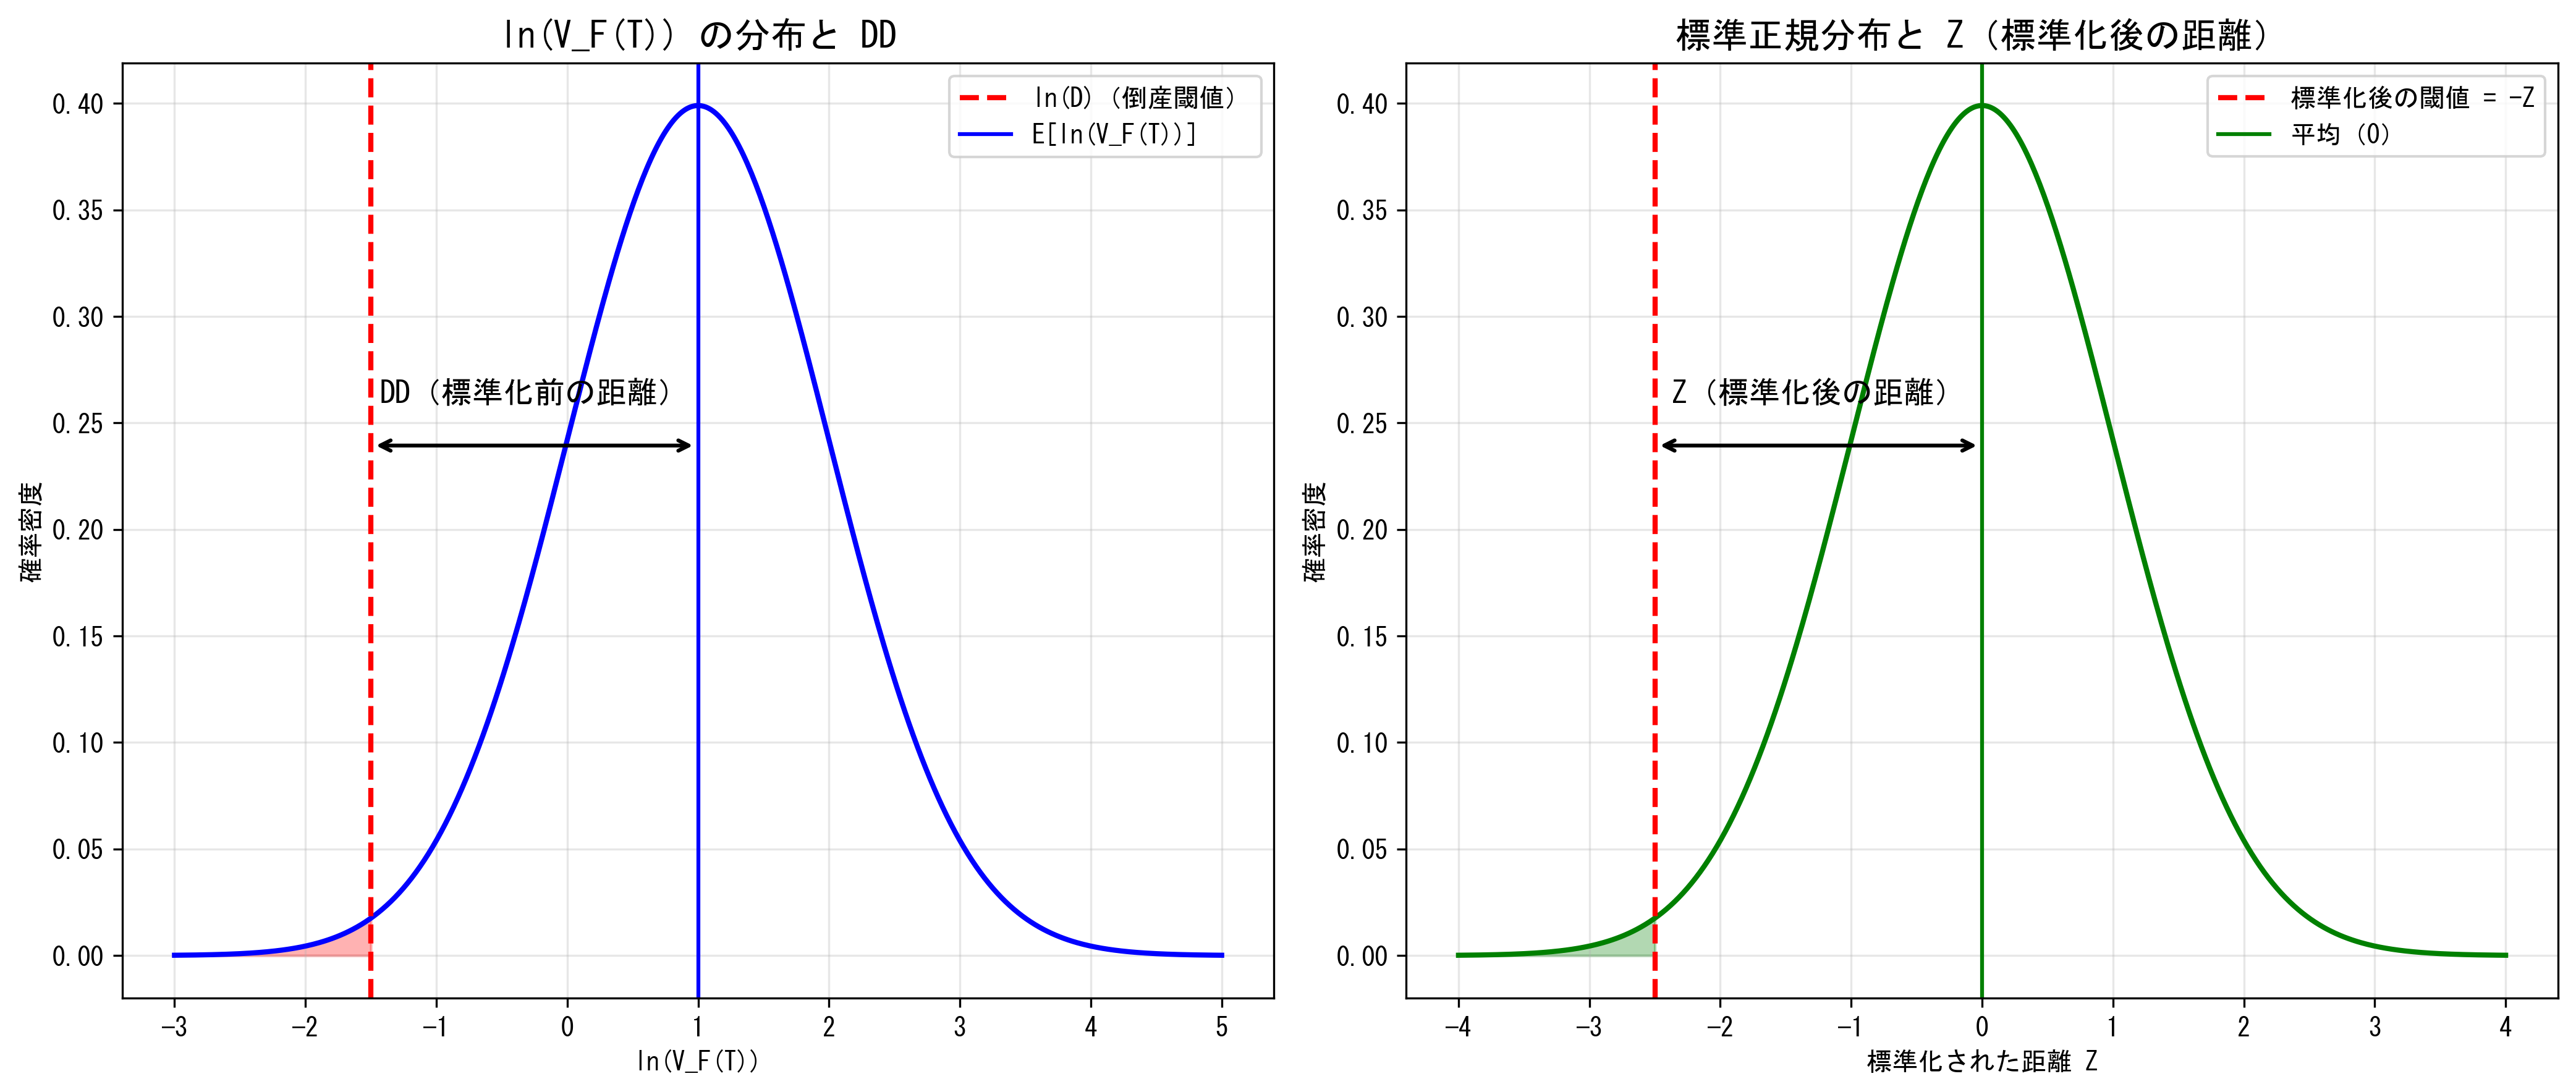
\includegraphics[width=0.85\linewidth]{figures/Bankruptcy_probability_of_Merton_model_with_Z.png}
\caption{
左図は $\ln V_F(T)$ の正規分布における倒産閾値 $\ln D$ と平均 $\mathbb{E}[\ln V_F(T)]$ の距離 DD を示す。
右図は標準正規分布に写像された倒産閾値 $z$ と平均 0 の距離 $z$ を示す。
両図は Merton モデルにおける倒産確率の決定構造（DD → $z$ → $\Phi(-z)$）を視覚的に示している。
}
\end{figure}

\section*{A.2　倒産閾値の標準正規分布への写像}
\addcontentsline{toc}{section}{A.2 倒産閾値の標準正規分布への写像}

Figure 1 の左図では、横軸は $x = \ln V_F(T)$ であり、倒産閾値は



\[
x = \ln D
\]



である。ここで $\ln V_F(T)$ の平均と分散を



\[
\mu_F = \mathbb{E}[\ln V_F(T)], \qquad 
\sigma_F^2 = \mathrm{Var}[\ln V_F(T)]
\]



とおく。

右図は、この分布を標準正規分布へ写像したものであり、横軸は



\[
z = \frac{x - \mu_F}{\sigma_F}
\]



で定義される標準化変数である。したがって倒産閾値 $x = \ln D$ は



\[
z = \frac{\ln D - \mu_F}{\sigma_F}
\]



へと写像される。

一方、倒産距離 DD は



\[
DD = \frac{\mu_F - \ln D}{\sigma_F}
\]



で定義されるため、標準正規分布の座標系では



\[
Z = -DD
\]



と置くことで、倒産方向への距離として解釈できる。

この標準化により、倒産確率は



\[
P(\text{default}) = \Phi(-Z)
\]



として表される。

\section*{A.3　本研究モデルとの対応関係}

本研究では、Merton モデルの構造を財務健全性スコア $F$ と倒産閾値 $\mathrm{Thr}$ に写像することで、
新電力企業の財務データに適用可能な倒産距離モデルを構築する。
このアプローチは Bharath \& Shumway（2008）が示した
「Merton モデルの proxy 化」という考え方を継承している。

\subsection*{（1）財務健全性 $H$ と対数変換 $F$}

本研究では、企業の財務状態を multiplicative に規定する量を「財務健全性」$H$ と定義する。
$H$ は収益性 $\mu$、外部ショック耐性 $\sigma$、支援能力 $S$ など複数の要因が掛け算的に作用する量である。



\[
H = H(\mu, \sigma, S)
\]



multiplicative な構造をもつ $H$ に対して対数変換を施すことで、additive な財務健全性スコア $F$ を得る。



\[
F = \ln H
\]



additive な $F$ は複数要因の和として表現されるため、中心極限定理により正規分布に従うとみなすことができる。

\subsection*{（2）倒産閾値 $\mathrm{Thr}$ の導入}

Merton モデルの倒産閾値 $\ln D$ に対応する量として、財務データに基づき設定される閾値 $\mathrm{Thr}$ を導入する。
財務健全性が閾値を下回る場合に倒産が発生するとみなし、



\[
F \le \mathrm{Thr}
\]



を倒産条件とする。

\subsection*{（3）倒産距離と標準化距離}

倒産距離（Distance to Default, DD）は



\[
DD = F - \mathrm{Thr}
\]



として定義される。さらに、$F$ の標準偏差 $\sigma_F$ で割ることで標準化距離 $Z$ が得られる。



\[
Z = \frac{DD}{\sigma_F}
\]



標準化距離 $Z$ は標準正規分布に従うため、倒産確率は



\[
\pi = \Phi(-Z)
\]



として与えられる。

\begin{figure}[H]
\centering
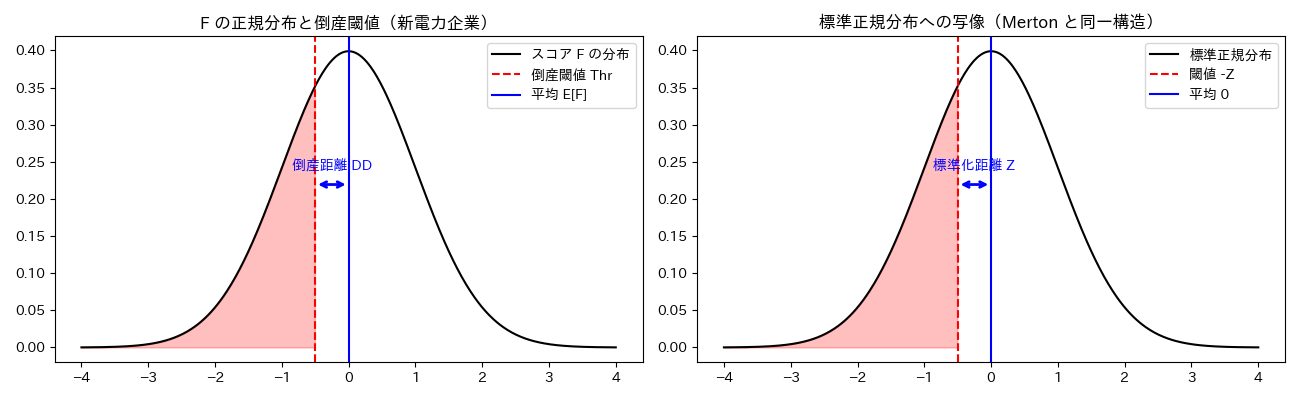
\includegraphics[width=0.95\linewidth]{figures/Bankruptcy_probability_of_New_Power_sec1.png}
\caption{
左図は multiplicative な財務健全性 $H$ を対数変換した財務健全性 $F=\ln H$ の正規分布と倒産閾値 $\mathrm{Thr}$ の関係を示す。
右図は標準正規分布への写像を示し、標準化距離 $Z = DD / \sigma_F$ と倒産確率 $\Phi(-Z)$ の構造が
Merton モデルと同一であることを示している。
}
\end{figure}

\subsection*{（4）対応関係の整理}

\begin{table}[H]
\centering
\begin{tabular}{lll}
\toprule
観点 & Merton モデル & 本研究 \\
\midrule
正規分布に従う変数 & $\ln V_F(T)$ & $F = \ln H$ \\
倒産閾値 & $\ln D$ & $\mathrm{Thr}$ \\
倒産距離（DD） & $E[\ln V_F(T)] - \ln D$ & $F - \mathrm{Thr}$ \\
標準化距離（Z） & $DD / \sigma_{\ln V}$ & $DD / \sigma_F$ \\
倒産確率 & $\Phi(-Z)$ & $\Phi(-Z)$ \\
経済的要因 & $V_F, D, \sigma_V$ & $\mu, \sigma, S$ \\
役割 & 分布を規定 & $H$ の multiplicative 構造を規定 \\
\bottomrule
\end{tabular}
\end{table}

%\appendix
